% Layout adapted from the research memo shown in Lecture 1, sized for A4.
\documentclass[a4paper,10pt]{article}
\usepackage[margin=18mm,footskip=9mm]{geometry}
\usepackage{iftex}
\ifPDFTeX
  \usepackage[T1]{fontenc}
  \usepackage[utf8]{inputenc}
  \usepackage[scaled=0.96]{helvet}
  \renewcommand{\familydefault}{\sfdefault}
\else
  \usepackage{fontspec}
  \setmainfont{texgyreheros}[Extension=.otf,
    UprightFont=*-regular, BoldFont=*-bold,
    ItalicFont=*-italic, BoldItalicFont=*-bolditalic]
\fi
\newif\ifChineseMemo
\ChineseMemofalse
\ifChineseMemo
  \ifPDFTeX
    \PackageError{finance-memo}{Chinese text requires XeLaTeX or LuaLaTeX}{}
  \else
    \usepackage[UTF8,fontset=fandol]{ctex}
    \renewcommand{\familydefault}{\sfdefault}
  \fi
\fi
\usepackage{booktabs,graphicx,xcolor,caption,xurl,fancyhdr}
\definecolor{MemoBlue}{HTML}{203E70}
\definecolor{MemoRule}{HTML}{B9C8DF}
\usepackage[colorlinks=true,linkcolor=MemoBlue,urlcolor=MemoBlue]{hyperref}
\captionsetup{font=small,labelfont=bf,skip=4pt}
\setlength{\parindent}{0pt}
\setlength{\parskip}{5pt}
\pagestyle{fancy}
\fancyhf{}
\renewcommand{\headrulewidth}{0pt}
\renewcommand{\footrulewidth}{0.3pt}

\newcommand{\ReportTitle}{Mega-cap technology: scale, growth and margin}
\newcommand{\ReportType}{RESEARCH MEMO}
\newcommand{\ReportDate}{31 October 2026}
\newcommand{\DataDate}{30 September 2026}
\newcommand{\ReportScope}{Latest five annual 10-K periods per company | USD | GAAP actuals}
\newcommand{\TeamName}{Equity Research}
\newcommand{\DeskName}{Mega-cap technology}
\newcommand{\ReportAuthor}{Kimi Code | Finance analysis}
\newcommand{\Coverage}{AAPL, MSFT, NVDA, GOOGL, AMZN}
\newcommand{\KeyFinding}{Amazon leads latest-year revenue scale; NVIDIA leads both revenue growth and GAAP net margin.}
\fancyfoot[L]{\scriptsize\TeamName}
\fancyfoot[C]{\scriptsize\thepage\ / 2}
\fancyfoot[R]{\scriptsize\ReportType}

\begin{document}
\begin{minipage}[t]{0.70\textwidth}
\vspace{0pt}
{\small\ReportDate}\par\medskip
{\color{MemoBlue}\hrule height 0.5pt}\smallskip
{\large\ReportType}\par\smallskip
{\LARGE\bfseries\ReportTitle}\par\medskip
\ReportScope
\end{minipage}\hfill
\begin{minipage}[t]{0.23\textwidth}
\vspace{0pt}\raggedleft
\colorbox{MemoBlue}{\parbox[c][19mm][c]{0.86\linewidth}{\centering\color{white}\bfseries\TeamName}}\par\medskip
\DeskName
\end{minipage}
\par\bigskip
{\color{MemoBlue}\hrule height 0.5pt}\medskip
{\large\KeyFinding}\par\bigskip

\begin{minipage}[t]{0.57\textwidth}
\vspace{0pt}\raggedright
\setlength{\parskip}{4pt}
\textbf{Scope}\par
The comparison covers the latest five fiscal years in original 10-K filings, with both fiscal-year end and filing date on or before the cutoff. Revenue growth is current-year revenue divided by prior-year revenue, minus one. Net margin is GAAP NetIncomeLoss attributable to parent divided by revenue. No estimates or non-GAAP adjustments are used.

\textbf{Findings}\par
Amazon's \$716.9bn revenue base is 72\% larger than Apple's \$416.2bn, the next-largest latest-year figure. NVIDIA's 65.5\% growth is well ahead of Microsoft's 17.8\%, while its 55.6\% net margin exceeds every peer.

The five-year history shows the scale of NVIDIA's shift: revenue rose from \$26.9bn in FY2022 to \$215.9bn in FY2026, and net margin moved from 16.2\% in FY2023 to 55.6\% in FY2026. Amazon's margin recovered from a 0.5\% loss in FY2022 to 10.8\% in FY2025. Apple's FY2023 revenue decline of 2.8\% is retained in the series.

\textbf{Interpretation}\par
These are reported operating outcomes, not causal estimates or investment recommendations. Scale, growth and margin rank different companies at the top and should be read separately.
\end{minipage}\hfill
\begin{minipage}[t]{0.40\textwidth}
\vspace{0pt}\small
\captionof{table}{Latest eligible fiscal year}\label{tab:latest}
{\footnotesize Revenue in USD billions; growth and net margin in percent.\par}
{\scriptsize\setlength{\tabcolsep}{3pt}\begin{tabular}{@{}llrrr@{}}
\toprule
Company & FY end & Revenue & Growth & Margin \\
 & & (\$bn) & (\%) & (\%) \\
\midrule
AAPL FY2025 & 2025-09-27 & 416.2 & 6.4 & 26.9 \\
MSFT FY2026 & 2026-06-30 & 331.8 & 17.8 & 40.3 \\
NVDA FY2026 & 2026-01-25 & 215.9 & 65.5 & 55.6 \\
GOOGL FY2025 & 2025-12-31 & 402.8 & 15.1 & 32.8 \\
AMZN FY2025 & 2025-12-31 & 716.9 & 12.4 & 10.8 \\
\bottomrule
\end{tabular}
\par}
{\footnotesize Source: original SEC 10-K XBRL facts. Fiscal-year ends are shown in ISO format.\par}


\textbf{Fiscal-calendar caution}\par
Latest periods end 27 Sep 2025 for Apple, 30 Jun 2026 for Microsoft, 25 Jan 2026 for NVIDIA, and 31 Dec 2025 for Alphabet and Amazon. They do not cover identical economic windows. Fiscal years can also span 52 or 53 weeks.

\textbf{Net-income caution}\par
GAAP net income can include tax, investment and other non-operating effects. Margin changes should not be interpreted as pure operating-margin changes without further statement analysis.
\end{minipage}
\par\medskip
\captionof{figure}{Latest-year scale, growth and profitability}\label{fig:latest}
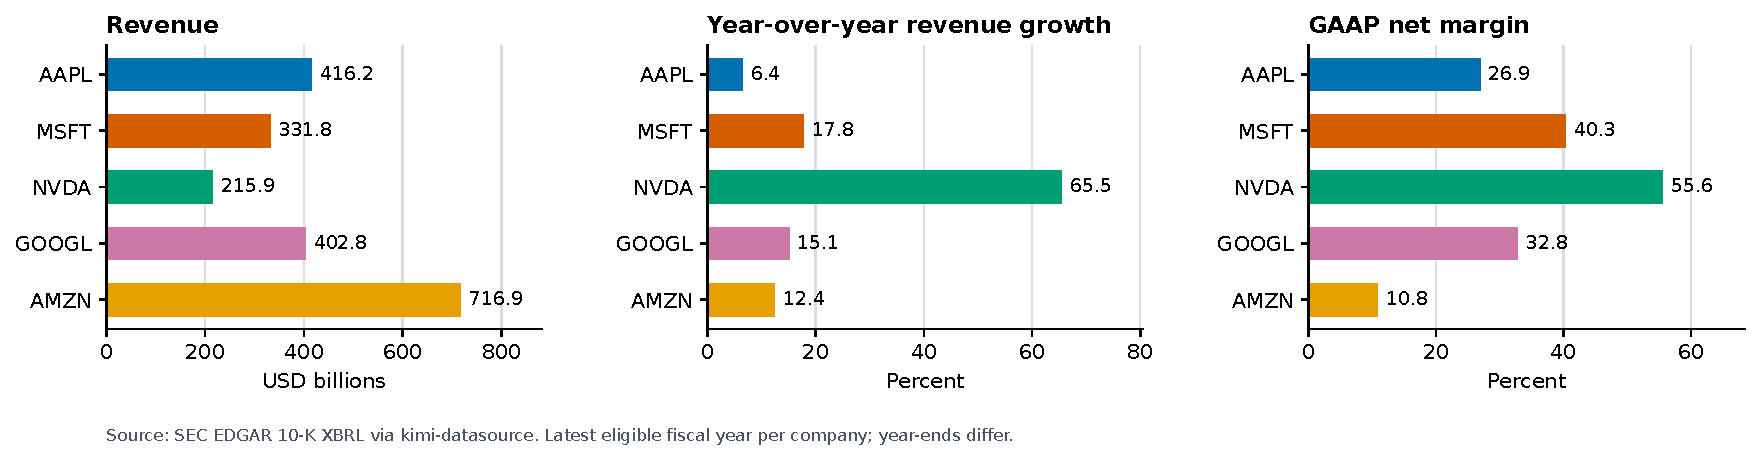
\includegraphics[width=\textwidth]{../output/figures/latest_fiscal_year_metrics.pdf}
{\footnotesize Latest eligible fiscal year per company; periods are not calendar-aligned. Values match Table \ref{tab:latest}.\par}

\vfill

{\color{MemoRule}\hrule height 0.4pt}\medskip
\begin{minipage}[t]{0.36\textwidth}
\vspace{0pt}\small
\setlength{\parskip}{3pt}
\textbf{PREPARED BY}\par\ReportAuthor\par\TeamName\par
\medskip\textbf{COVERAGE}\par\Coverage
\end{minipage}\hfill
\begin{minipage}[t]{0.60\textwidth}
\vspace{0pt}\footnotesize
\setlength{\parskip}{3pt}
\textbf{Sources and dates.} SEC EDGAR 10-K filings and XBRL facts via kimi-datasource; cutoff \DataDate. Original accessions are linked on page 2. Raw extracts are preserved under \path{data/raw/sec_edgar/}.

\textbf{Checks.} All 25 annual rows passed accession, period, unit and calculation checks. Verification is reconciliation to retained source records, not independent re-audit.
\end{minipage}

\clearpage
{\color{MemoBlue}\hrule height 0.5pt}\medskip
{\large\ReportType}\par\smallskip
{\LARGE\bfseries Annual history and audit trail}\par\medskip
\textbf{Annual comparison.} Five fiscal years per company; revenue in USD billions, growth and net margin in percent. Negative values are reported outcomes, not missing data.
\captionof{table}{Five-year annual comparison}\label{tab:annual}
{\footnotesize Source: SEC EDGAR 10-K XBRL facts via kimi-datasource. Growth uses the preceding fiscal year; net margin uses GAAP NetIncomeLoss / revenue.\par}
{\footnotesize\setlength{\tabcolsep}{5pt}\begin{tabular}{@{}lllrrr@{}}
\toprule
Ticker & FY & Fiscal-year end & Revenue (\$bn) & Growth (\%) & Net margin (\%) \\
\midrule
AAPL & 2021 & 2021-09-25 & 365.8 & 33.3 & 25.9 \\
AAPL & 2022 & 2022-09-24 & 394.3 & 7.8 & 25.3 \\
AAPL & 2023 & 2023-09-30 & 383.3 & -2.8 & 25.3 \\
AAPL & 2024 & 2024-09-28 & 391.0 & 2.0 & 24.0 \\
AAPL & 2025 & 2025-09-27 & 416.2 & 6.4 & 26.9 \\
\addlinespace[2pt]
MSFT & 2022 & 2022-06-30 & 198.3 & 18.0 & 36.7 \\
MSFT & 2023 & 2023-06-30 & 211.9 & 6.9 & 34.1 \\
MSFT & 2024 & 2024-06-30 & 245.1 & 15.7 & 36.0 \\
MSFT & 2025 & 2025-06-30 & 281.7 & 14.9 & 36.1 \\
MSFT & 2026 & 2026-06-30 & 331.8 & 17.8 & 40.3 \\
\addlinespace[2pt]
NVDA & 2022 & 2022-01-30 & 26.9 & 61.4 & 36.2 \\
NVDA & 2023 & 2023-01-29 & 27.0 & 0.2 & 16.2 \\
NVDA & 2024 & 2024-01-28 & 60.9 & 125.9 & 48.8 \\
NVDA & 2025 & 2025-01-26 & 130.5 & 114.2 & 55.8 \\
NVDA & 2026 & 2026-01-25 & 215.9 & 65.5 & 55.6 \\
\addlinespace[2pt]
GOOGL & 2021 & 2021-12-31 & 257.6 & 41.2 & 29.5 \\
GOOGL & 2022 & 2022-12-31 & 282.8 & 9.8 & 21.2 \\
GOOGL & 2023 & 2023-12-31 & 307.4 & 8.7 & 24.0 \\
GOOGL & 2024 & 2024-12-31 & 350.0 & 13.9 & 28.6 \\
GOOGL & 2025 & 2025-12-31 & 402.8 & 15.1 & 32.8 \\
\addlinespace[2pt]
AMZN & 2021 & 2021-12-31 & 469.8 & 21.7 & 7.1 \\
AMZN & 2022 & 2022-12-31 & 514.0 & 9.4 & -0.5 \\
AMZN & 2023 & 2023-12-31 & 574.8 & 11.8 & 5.3 \\
AMZN & 2024 & 2024-12-31 & 638.0 & 11.0 & 9.3 \\
AMZN & 2025 & 2025-12-31 & 716.9 & 12.4 & 10.8 \\
\bottomrule
\end{tabular}
\par}


\captionof{table}{Latest-year 10-K source records}\label{tab:sources}
{\footnotesize Accessions link to SEC filing indexes. The complete 30-period source record, including growth baselines and XBRL concepts, is retained in \path{output/tables/source_records.csv}.\par}
{\footnotesize\setlength{\tabcolsep}{5pt}\begin{tabular}{@{}llll@{}}
\toprule
Ticker & Fiscal-year end & Filed & 10-K accession \\
\midrule
AAPL & 2025-09-27 & 2025-10-31 & \href{https://www.sec.gov/Archives/edgar/data/320193/0000320193-25-000079-index.html}{0000320193-25-000079} \\
MSFT & 2026-06-30 & 2026-07-29 & \href{https://www.sec.gov/Archives/edgar/data/789019/0001193125-26-323660-index.html}{0001193125-26-323660} \\
NVDA & 2026-01-25 & 2026-02-25 & \href{https://www.sec.gov/Archives/edgar/data/1045810/0001045810-26-000021-index.html}{0001045810-26-000021} \\
GOOGL & 2025-12-31 & 2026-02-05 & \href{https://www.sec.gov/Archives/edgar/data/1652044/0001652044-26-000018-index.html}{0001652044-26-000018} \\
AMZN & 2025-12-31 & 2026-02-06 & \href{https://www.sec.gov/Archives/edgar/data/1018724/0001018724-26-000004-index.html}{0001018724-26-000004} \\
\bottomrule
\end{tabular}
\par}


\begin{minipage}[t]{0.49\textwidth}
\vspace{0pt}\small
\textbf{Method and definitions}\par
Original 10-K facts are selected by company, fiscal year, accession and fiscal-year end. Annual durations of 330--380 days are required; later comparative-filing duplicates are excluded. Revenue uses the consolidated reported annual value. Net income uses \texttt{us-gaap:NetIncomeLoss}. Calculations use unrounded USD inputs; displayed values are rounded to one decimal.

The source file contains 30 company-periods: the 25 displayed years plus one prior-year revenue baseline per company. Fiscal-year end dates, filing dates, concepts, accessions and SEC links remain attached to each source row.
\end{minipage}\hfill
\begin{minipage}[t]{0.48\textwidth}
\vspace{0pt}\small
\textbf{Verification status: PASS}\par
\begin{itemize}
\setlength{\itemsep}{1pt}
\setlength{\parskip}{0pt}
\item 25 annual rows; five years for each of five companies.
\item 30 retained source periods, including growth baselines.
\item USD, annual duration, 10-K form and original-accession checks passed.
\item Growth and net margin recomputed for every row; no missing values.
\item Latest-year revenue and net income matched separate structured income-statement extracts for all five firms.
\item Chart values and HTML tables generated from the same checked dataset.
\end{itemize}
\textbf{Reproducibility.} Run \path{python3 src/build_annual_comparison.py}. Checked outputs are in \path{output/tables/}; the full annual chart is in \path{output/figures/}. Preparation used AI assistance for retrieval, calculation and drafting.

\textbf{Limitations.} Fiscal periods are not calendar-aligned; no segment, tax or one-off normalization is attempted. AI-generated analysis; not investment advice.
\end{minipage}
\end{document}
